% D4 final report, COEN 424/6313 Programming on Cloud, Fall 2026, Group D.
% IEEE conference format (IEEEtran). Compile: pdflatex D4-report-GroupD.tex (twice).
\documentclass[conference]{IEEEtran}
\usepackage[utf8]{inputenc}
\usepackage[T1]{fontenc}
\usepackage{amsmath}
\usepackage{booktabs}
\usepackage{tabularx}
\usepackage{graphicx}
\usepackage{xcolor}
\usepackage{listings}
\usepackage{tikz}
\usetikzlibrary{arrows.meta,positioning,fit,shapes.geometric}
\usepackage[hidelinks]{hyperref}
\usepackage{url}

\lstset{basicstyle=\ttfamily\scriptsize,columns=fullflexible,frame=single,
  framerule=0.3pt,xleftmargin=2pt,xrightmargin=2pt,aboveskip=4pt,belowskip=4pt}
\newcolumntype{L}[1]{>{\raggedright\arraybackslash}p{#1}}
\newcolumntype{Y}{>{\raggedright\arraybackslash}X}
\newcommand{\todo}[1]{\textcolor{red}{[TODO: #1]}}

\begin{document}

\title{Safely Replacing a Microservice with an AI Agent:\\
A Canary Migration of Online Boutique on Azure}

\author{
\IEEEauthorblockN{Mustafa Ghouri (40355660), Nofil Siddiqui (40292948), Rahil Shah (40329714)}
\IEEEauthorblockA{COEN 424/6313 Programming on Cloud, Fall 2026, Group D (Option B)\\
Concordia University, Montr\'eal, Canada}
}

\maketitle

\begin{abstract}
We deployed Google's Online Boutique, an e-commerce application of eleven
gRPC microservices, on Azure Container Apps and replaced one component, the
recommendation service, with an AI agent. The original service (v1) returns
random products. The agent (v2) gives a language model the shopper's
products, the store's categories and a shortlist of candidates, lets it call
catalog tools, and validates its choice before answering. It falls back to
v1's behaviour on any failure. We redesigned the recommendation API so the
caller sets the number of results and every product carries a reason. The
change is backward compatible and implemented by both versions. Traffic is
moved from v1 to v2 with a strangler-pattern canary: Container Apps
revision traffic splitting, steps of 10, 25, 50 and 100\%, load from the
Online Boutique load generator, and four criteria fixed in advance
(availability, p95 latency, correctness, cost). The canary promoted v2 with
0\% errors, a p95 latency of 645--1362\,ms and 100\% correct responses. A
fault-injected v2 with an invalid model key was rolled back at the first
step. Its error rate was still 0\%, and only the correctness check caught
it. At list prices v2 costs about 1.45 times v1 per request. The actual bill
was \$0 because every service stayed within a free tier.
\end{abstract}

\begin{IEEEkeywords}
microservices, AI agents, canary release, strangler pattern, Azure Container Apps, gRPC, API evolution
\end{IEEEkeywords}

\section{Introduction}

\subsection{Goal}
Show that a component of a running cloud application can be replaced by an
AI agent \emph{safely}. The agent must keep the component's contract, be
introduced gradually, be measured against criteria fixed in advance, and be
withdrawn automatically when it misbehaves.

\subsection{Problem Statement}
Large language models make it attractive to turn rule-based services into
agents that reason about each request. An agent can fail in ways a
deterministic service does not. It can be slow, expensive per call, or
rate-limited. It can also return a response that is well-formed but wrong,
for example a product ID that does not exist or one the shopper already
owns. Such responses do not raise errors, so the usual availability
monitoring misses them. A migration therefore needs a facade that controls
which version serves each request, and criteria that test correctness as
well as errors and latency.

\subsection{Objectives}
\begin{enumerate}
\item Deploy Online Boutique~\cite{boutique} on a public cloud, using
platform-specific features: Azure Container Apps, revisions, and Cosmos DB.
\item Build an AI agent version (v2) of the recommendation service that
uses a model to choose and call tools, with a fallback to v1.
\item Redesign the recommendation API in a backward-compatible way and
implement it in both versions.
\item Canary traffic from v1 to v2 in at least three steps, with one
promotion and one rollback.
\item Monitor both versions on an Azure Monitor dashboard, and report cost
per request and total cost.
\end{enumerate}

\subsection{Assumptions}
\begin{itemize}
\item The shop's other ten services are used unchanged, except the frontend
(for the API change) and the product catalog (extended from 9 to 200
products in 24 categories, so recommendations can be meaningful).
\item All cloud resources run on an Azure for Students subscription with a
\$10 monthly budget. Free tiers are preferred wherever they exist.
\item The model is an open-weight model reached through an OpenAI-compatible
API, so the provider can be changed by configuration alone.
\item The load generator's traffic (two simulated shoppers) stands in for
real users. Results at production load may differ.
\end{itemize}

\subsection{Methodology}
We worked in phases, each ending in a pull request and a demo:
\begin{enumerate}
\item local Docker setup and a contract smoke test;
\item Azure foundation: budget and alerts before the first deployment,
Bicep templates and v1 on Container Apps;
\item the v2 agent, unit-tested against a scripted model;
\item canary tooling, criteria and measurements;
\item the API redesign, which answered the lecturer's feedback after the
first demo.
\end{enumerate}
Infrastructure is code (Bicep and shell scripts), and images are built by
GitHub Actions. AI coding assistants were used throughout. The prompts,
tools and models are logged in the repository under
\texttt{docs/ai-usage}, as the course requires.

\subsection{Schedule}
Table~\ref{tab:schedule} lists the milestones.

\begin{table}[t]
\caption{Schedule}
\label{tab:schedule}
\centering\small
\begin{tabularx}{\columnwidth}{@{}lY@{}}
\toprule
When & Milestone \\
\midrule
Week 2--3 & D1 group, D2 scope: Option B, recommendation service as agent, Azure \\
Week 6 (Oct.\ 23--26) & Local stack; v2 agent (local Qwen3-4B); v1 and Cosmos DB on Azure; D3 demo \\
Nov.\ 16 & v2 on Azure (Groq); canary scripts, criteria, measurements; dashboard; cost report \\
Nov.\ 16 & Recommendation API version 2 (lecturer's feedback) \\
Week 12 & D4 presentation, live demo, report \\
\bottomrule
\end{tabularx}
\end{table}

\section{Project Description}

\subsection{Function Provided by the Service}
Online Boutique is a web shop: browse products, convert currency, manage a
cart and check out. The recommendation service fills the ``You May Also
Like'' box on product, cart and order pages. Given the shopper's products,
it returns other products to show. v1 picks at random. v2 asks a language
model to choose complementary products, and explains each choice to the
shopper (for example, Gooseneck Kettle: ``Perfect for brewing with your
mug''). Any client can call the service through its gRPC API (Section~\ref{sec:api}).

\subsection{Architectural Design}
Fig.~\ref{fig:arch} shows the deployment. Each microservice is an Azure
Container App in one Container Apps environment. Only the frontend has
public HTTPS ingress. The other services talk plaintext gRPC over the
environment's internal network. The cart uses a Redis sidecar.

\begin{figure*}[t]
\centering
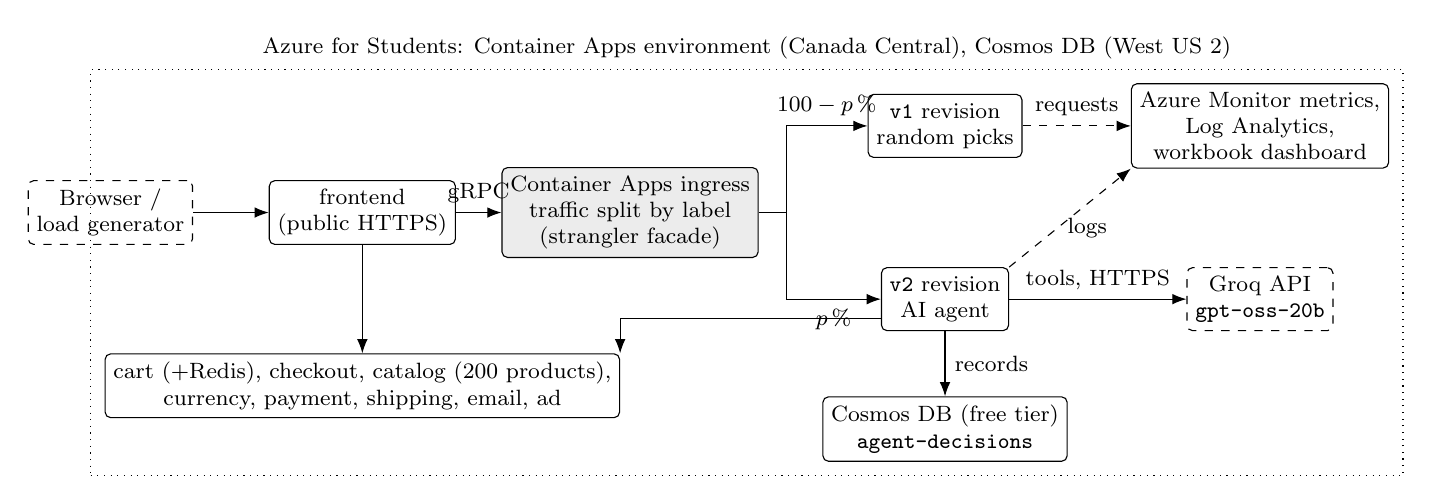
\begin{tikzpicture}[font=\footnotesize,
  box/.style={draw,rounded corners=2pt,align=center,minimum height=8mm,inner sep=3pt},
  ext/.style={box,dashed},
  arr/.style={-{Latex[length=1.8mm]}}]
\node[ext] (user) at (0,0) {Browser /\\load generator};
\node[box] (fe) at (3.2,0) {frontend\\(public HTTPS)};
\node[box,fill=gray!15] (facade) at (6.6,0) {Container Apps ingress\\traffic split by label\\(strangler facade)};
\node[box] (v1) at (10.6,1.1) {\texttt{v1} revision\\random picks};
\node[box] (v2) at (10.6,-1.1) {\texttt{v2} revision\\AI agent};
\node[box] (others) at (3.2,-2.2) {cart (+Redis), checkout, catalog (200 products),\\currency, payment, shipping, email, ad};
\node[box] (cosmos) at (10.6,-2.75) {Cosmos DB (free tier)\\\texttt{agent-decisions}};
\node[box] (mon) at (14.6,1.1) {Azure Monitor metrics,\\Log Analytics,\\workbook dashboard};
\node[ext] (groq) at (14.6,-1.1) {Groq API\\\texttt{gpt-oss-20b}};
\draw[arr] (user) -- (fe);
\draw[arr] (fe) -- node[above]{gRPC} (facade);
\draw[arr] (facade.east) -- ++(0.35,0) |- node[pos=0.75,above]{$100-p\,\%$} (v1.west);
\draw[arr] (facade.east) -- ++(0.35,0) |- node[pos=0.75,below]{$p\,\%$} (v2.west);
\draw[arr] (fe) -- (others);
\draw[arr] (v2) -- node[above]{tools, HTTPS} (groq);
\draw[arr] (v2) -- node[right]{records} (cosmos);
\draw[arr] (v2.west) ++(0,-0.25) -| (others.north east);
\draw[arr,dashed] (v1) -- node[above]{requests} (mon);
\draw[arr,dashed] (v2.north east) -- node[right,pos=0.4]{logs} (mon.south west);
\node[draw,dotted,inner sep=5pt,fit=(fe)(facade)(v1)(v2)(others)(cosmos)(mon),
  label={[font=\footnotesize]above:{Azure for Students: Container Apps environment (Canada Central), Cosmos DB (West US 2)}}] {};
\end{tikzpicture}
\caption{Deployment. Each microservice is a Container App. The recommendation
service runs two labelled revisions behind one internal endpoint, and the
ingress splits requests between them by the canary's weight $p$. v2 calls
the model and the catalog, and records every decision. Dashed: external
service and telemetry.}
\label{fig:arch}
\end{figure*}

\textbf{Strangler facade.} The strangler pattern~\cite{fowler-strangler}
replaces a system piece by piece behind a facade that decides which
implementation serves each request. Our facade is Container Apps' revision
traffic splitting~\cite{aca-traffic}. The recommendation app runs in
\emph{multiple-revision} mode. The v1 and v2 revisions carry the labels
\texttt{v1} and \texttt{v2}, and the ingress weights decide each request.
The frontend always calls \texttt{recommendationservice:80}, so it cannot
tell which version answered.

\textbf{Data model.} Products are a read-only JSON catalog in the catalog
image. Carts are key--value pairs in Redis (\texttt{userId}~$\rightarrow$
items and quantities). Orders are not stored: they are charged, e-mailed
(both mocked) and discarded. Prices use a \texttt{Money} type of whole
units plus nanos, which avoids floating-point rounding. v2 adds one
document per response to a free-tier Cosmos DB container. The document holds
the context, recommended IDs and their reasons, the outcome
(\texttt{agent}, \texttt{cached} or \texttt{fallback}), the model, tokens
and latency. The partition key is \texttt{/userId}, and a 30-day TTL keeps
storage inside the free tier. Writes are asynchronous, so a slow database
never delays a recommendation. The agent keeps no conversation: each
request is one stateless exchange. An in-memory cache (10 minutes, keyed by
the sorted context and \texttt{max\_results}) reuses recent decisions.
Table~\ref{tab:record} lists the fields of a decision record.

\begin{table}[t]
\caption{v2 decision record in Cosmos DB (one per response)}
\label{tab:record}
\centering\footnotesize
\begin{tabularx}{\columnwidth}{@{}L{0.47\columnwidth}Y@{}}
\toprule
Field & Meaning \\
\midrule
\texttt{id}, \texttt{userId} & document ID; shopper session (partition key) \\
\texttt{timestamp}, \texttt{version} & when; \texttt{v2} \\
\texttt{contextProductIds} & request: viewed product and cart \\
\texttt{recommendedProductIds} & response, in order \\
\texttt{productReasons} & reason per product (API version 2) \\
\texttt{outcome} & \texttt{agent}, \texttt{cached} or \texttt{fallback} \\
\texttt{fallbackReason}, \texttt{reason} & why the model was bypassed; the model's summary \\
\texttt{toolCalls}, \texttt{steps}, \texttt{toppedUp} & tools called, model calls, random fill \\
\texttt{model}, \texttt{promptTokens}, \texttt{completionTokens} & model and usage (the cost driver) \\
\texttt{latencyMs} & time to answer \\
\bottomrule
\end{tabularx}
\end{table}

\subsection{Technical Implementation}

\textbf{AI agent (v2).} The agent is written in Python with gRPC. It sends
the model the shopper's products, the store's categories and a shortlist
of 12 related candidates, and exposes four tools: \texttt{browse\_category},
\texttt{search\_catalog}, \texttt{get\_products} and \texttt{recommend}
(the final answer, with a reason per product). This is the tool-use pattern
of ReAct~\cite{react} and Toolformer~\cite{toolformer}. The model decides
which products to return, so v2 is an agent rather than a model that
rephrases v1's output. Guardrails drop IDs that are unknown, duplicated or
already owned, and cap the list. If fewer products remain than requested,
the list is topped up at random. If the model fails, times out or returns
nothing usable, the agent answers with v1's random choice. The client
therefore always receives a valid response. Thirty-two unit tests run
against a scripted model, and the image build runs them.

\textbf{Model.} The Hugging Face free account had no inference credits. We
therefore first ran Qwen3-4B-Instruct~\cite{qwen3} locally with Ollama: the
choices were relevant, but each took 20--60\,s on a laptop CPU. On Azure,
v2 uses \texttt{openai/gpt-oss-20b}~\cite{gptoss} on Groq's free
plan~\cite{groq} in single-step mode (the model calls \texttt{recommend}
directly, with low reasoning effort). A local check of five cases gave 5/5
model decisions with a p95 of 924\,ms. The provider is configuration only:
a base URL, a model name and a key held as a Container Apps secret, never in
the repository.

\textbf{Recommendation API version 2.}\label{sec:api} After our first demo,
the lecturer asked us to design the interface ourselves rather than reuse
Google's unchanged. Version 2 adds two things to the Protocol Buffers
contract:

\begin{lstlisting}
message ListRecommendationsRequest {
  string user_id = 1;
  repeated string product_ids = 2;
  int32 max_results = 3;   // NEW: 1-10, 0 = default 5
}
message ListRecommendationsResponse {
  repeated string product_ids = 1;  // kept for v1 clients
  repeated Recommendation recommendations = 2; // NEW
}
message Recommendation { string product_id = 1;
                         string reason = 2; }  // NEW
\end{lstlisting}

The caller states how many recommendations it can show. The frontend used
to discard the fifth; it now asks for four. Each product carries a reason,
so the shopper sees why it is suggested. The change only adds fields. No
field is renamed, renumbered or removed, so Protobuf's rules for unknown and
default fields~\cite{protobuf} keep every client--server combination
working (Table~\ref{tab:compat}). \emph{Both} implementations
use version~2: v1 gives a rule-based reason (``From our kitchen
collection''), v2 the model's own. The project description asks the agent
to keep the replaced component's interface unchanged; we therefore changed
the API once, before the canary, for both versions together. During the
canary v1 and v2 expose the same contract, so a client still cannot tell
which version served a request. We built v1 from Google's
source with this change, and the frontend from source to show the reasons.
Each service's stubs were generated with the tool version that matches its
Protobuf runtime.

\begin{table}[t]
\caption{Compatibility of the API versions}
\label{tab:compat}
\centering\small
\begin{tabularx}{\columnwidth}{@{}llY@{}}
\toprule
Client & Server & Result \\
\midrule
v1 (Google) & v2 (ours) & \texttt{max\_results}${}=0$, so the default of 5 applies; client reads \texttt{product\_ids} \\
v2 (ours) & v1 (Google) & 5 IDs, no reasons; frontend keeps 4, shows no reason line \\
v2 & v2 & 4 products, each with a reason \\
v1 & v1 & unchanged \\
\bottomrule
\end{tabularx}
\end{table}

\textbf{Infrastructure and CI/CD (extra feature).} Bicep templates define
Log Analytics (capped at 0.15\,GB/day), the Container Apps environment, the
ten apps and Cosmos DB. A budget with alerts at 50/80/100\% was created
before the first deployment. Resources are tagged with \texttt{project},
\texttt{component} and \texttt{version}. Tags apply to a whole app, not to a
revision, so v1's and v2's compute is split by each revision's Azure Monitor
usage instead (Section~\ref{sec:cost}). A GitHub Actions workflow builds
the four images we change (v1, v2, catalog, frontend) and pushes them to
GitHub Container Registry with commit, branch and \texttt{latest} tags.
\texttt{cloud.sh} stops and starts the whole shop between demos.
\texttt{canary.sh} deploys revisions and drives the canary.

\textbf{Security and cost guardrails.} The repository holds no
credentials. The model key and the Cosmos DB key are Container Apps secrets,
set by the deployment script from a git-ignored local file or a hidden
prompt. Every script pins the Azure for Students subscription before it
acts, and refuses to deploy before the budget exists. Internal services have
no public endpoint. The Cosmos DB account is created only if the
subscription's free tier is still unused, so the scripts never create a
billed account by accident.

\subsection{Migration Method and Comparison}

\textbf{Criteria.} Before the first canary we fixed the criteria in
Table~\ref{tab:criteria}~\cite{sre-canary}. At each step v2 is judged under
the load generator's traffic~\cite{locust}. Availability comes from the
Azure Monitor \texttt{Requests} metric per revision (HTTP 5xx) and from v2's
records of failed requests, because a non-OK gRPC status reaches the
platform as HTTP 200. Latency, correctness
and tokens come from v2's decision records. A response is \emph{correct}
when the model made the choice (\texttt{agent} or \texttt{cached}, not a
fallback), every ID exists, there are no duplicates or owned products, the
count is within \texttt{max\_results}, and every product has a reason.
Container Apps reports response time per app, not per revision, so the
latency threshold judges v2 on its own. To compare with v1 under the same
load, each step also records the p95 of whole shop pages from the load
generator. v1 needs only one catalog call and no model call.

\begin{table}[t]
\caption{Canary criteria (fixed in advance; violation $\Rightarrow$ roll back to v1)}
\label{tab:criteria}
\centering\small
\begin{tabularx}{\columnwidth}{@{}lYl@{}}
\toprule
Metric & Measured as & v2 threshold \\
\midrule
Availability & 5xx, timeouts and gRPC errors / requests, per revision & $\le$1\%, $\le$v1+1 pt \\
Latency & p95 of v2 \texttt{latencyMs} over the step & $\le$2000\,ms \\
Correctness & share of v2 responses passing all rules & $\ge$95\% \\
Cost & tokens per model call; Azure spend & $\le$1500; $<$\$8 \\
\bottomrule
\end{tabularx}
\end{table}

\textbf{Procedure.} \texttt{canary.sh run} sets the v2 share to 10, 25, 50
and 100\%. At each step it applies five minutes of load (two simulated
shoppers, sized for Groq's free limits of 8000 tokens per minute and 1000
requests per day). It then waits three minutes, because Azure Monitor
time-stamps requests 1--2 minutes late, and runs the checker. If every
criterion passes, the canary moves to the next step. If any fails, it sends
all traffic back to v1 (Fig.~\ref{fig:canary}).

\begin{figure}[t]
\centering
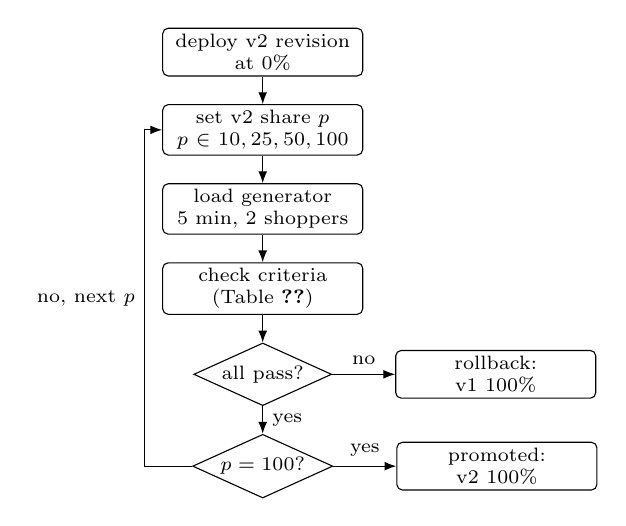
\begin{tikzpicture}[font=\scriptsize,node distance=3.5mm,
  box/.style={draw,rounded corners=2pt,align=center,minimum height=6mm,inner sep=2pt,text width=24mm},
  dec/.style={draw,diamond,aspect=2.2,align=center,inner sep=1pt},
  arr/.style={-{Latex[length=1.5mm]}}]
\node[box] (dep) {deploy v2 revision\\at 0\%};
\node[box,below=of dep] (set) {set v2 share $p$\\$p \in 10,25,50,100$};
\node[box,below=of set] (load) {load generator\\5 min, 2 shoppers};
\node[box,below=of load] (chk) {check criteria\\(Table~\ref{tab:criteria})};
\node[dec,below=of chk] (ok) {all pass?};
\node[box,right=8mm of ok] (rb) {rollback:\\v1 100\%};
\node[dec,below=of ok] (last) {$p=100$?};
\node[box,right=8mm of last] (pro) {promoted:\\v2 100\%};
\draw[arr] (dep) -- (set);
\draw[arr] (set) -- (load);
\draw[arr] (load) -- (chk);
\draw[arr] (chk) -- (ok);
\draw[arr] (ok) -- node[above]{no} (rb);
\draw[arr] (ok) -- node[right]{yes} (last);
\draw[arr] (last) -- node[above]{yes} (pro);
\draw[arr] (last.west) -- ++(-0.6,0) |- node[pos=0.25,left]{no, next $p$} (set.west);
\end{tikzpicture}
\caption{The canary run (\texttt{canary.sh run}).}
\label{fig:canary}
\end{figure}

\begin{table}[t]
\caption{Canary run 1: promotion of v2}
\label{tab:promotion}
\centering\small
\begin{tabular}{@{}rrrrrr@{}}
\toprule
v2 share & Req.\ v1/v2 & Errors & p95 & Correct & Tokens \\
\midrule
10\% & 103/11 & 0\% & 840\,ms & 100\% & 822 \\
25\% & 78/29 & 0\% & 1362\,ms & 100\% & 854 \\
50\% & 60/58 & 0\% & 902\,ms & 100\% & 805 \\
100\% & 0/114 & 0\% & 645\,ms & 100\% & 799 \\
\bottomrule
\end{tabular}
\end{table}

\textbf{Promotion.} Table~\ref{tab:promotion} shows the first run. v2 met
every criterion at every step and was promoted. Only 45 of 212 v2 requests
needed a model call; the rest reused a cached decision, because the load
generator visits only nine products. After the API change, a two-minute step
at 50\% again passed every criterion (p95 658\,ms, 100\% correct including
the reason rule, 864 tokens per model call).

\textbf{Rollback.} We deployed a v2 with an invalid model key and ran the
canary again. At 10\%, all 11 v2 responses were fallbacks: correctness 0\%,
so the canary rolled back to v1 automatically. Availability \emph{passed}
(0\% errors), and latency was the lowest observed (p95 249\,ms), because a
fallback answers immediately. Error rate alone would have promoted this
faulty agent. Only the correctness criterion caught it, as the project
description warns.

\textbf{Comparison.} v1 answers without a model, while v2 adds a model call
of about 0.3--1.4\,s. v2's p95 stayed within the 2\,s threshold, and the
shop's page p95 was 0.9--1.3\,s at every step. In quality, v1's
recommendations are random (a mug next to loafers), while v2's are
complementary (mug $\rightarrow$ French press, gooseneck kettle, espresso
cups), with a reason for each.

\textbf{Monitoring.} An Azure Monitor workbook, deployed from Bicep, shows
requests per revision (the traffic split over time), status codes, v2's
p95, outcomes (agent, cached or fallback) and tokens per model call.

\subsection{Cost Report}
The actual bill was \textbf{\$0.00}. Cost Management showed no charge for
the month, because every service stayed within a free allowance: Container
Apps' monthly grant~\cite{aca-billing}, Cosmos DB's free tier~\cite{cosmos-free},
capped Log Analytics, and Groq's free plan. To compare the two versions, we
priced the canary day's measured usage at list prices: Canada Central
\$0.000034 per vCPU-second, \$0.000004 per GiB-second, and \$0.40 per
million requests; Groq \$0.075/\$0.30 per million input/output tokens.
Each revision runs one 0.25\,vCPU / 0.5\,GiB replica, which costs
\$0.00063 per minute.

\begin{table}[t]
\caption{Cost of v1 and v2 on the canary day at list prices}
\label{tab:cost}
\centering\small
\begin{tabular}{@{}lrr@{}}
\toprule
 & v1 & v2 \\
\midrule
Requests served & 393 & 269 \\
Replica-minutes & 60 & 50 \\
Model calls / tokens (in+out) & -- & 59 / 48{,}241 \\
Compute + requests & \$0.0380 & \$0.0316 \\
Model & -- & \$0.0060 \\
\textbf{Cost per request} & \textbf{\$0.000097} & \textbf{\$0.000140} \\
\bottomrule
\end{tabular}
\end{table}

Table~\ref{tab:cost} gives the result: v2 costs about 1.45 times v1 per
request. At this light load, idle compute dominates both versions. The model
adds \$0.0000224 per request on average (\$0.0001 per call), because the
cache answered 210 of 269 requests. Without the cache, model cost per
request would be about 4.5 times higher. At one million requests a month
the model would cost about \$22 with the cache, or \$102 without it.

\subsection{Source Code and Service}
\noindent Source code:\\
\url{https://github.com/POC-Group-D/POC-Term-Project}\\[2pt]
Service (kept stopped between demos to save credit; started on request):\\
\url{https://frontend.blueflower-54b52d82.canadacentral.azurecontainerapps.io}

\section{Discussion}

\textbf{Correctness is the criterion that matters for agents.} The faulty
agent was fast and error-free, yet useless. A canary that judges an agent
only on errors and latency can promote a broken agent. Checking each
response against explicit rules, and counting fallbacks as failures, turned
a silent fault into an automatic rollback.

\textbf{Fallbacks protect users but hide problems.} The fallback kept the
shop working when the model failed, but from the outside the failure was
invisible. It must be measured separately; we record an \texttt{outcome}
field for every decision.

\textbf{Model hosting is the main constraint.} Hugging Face's free account
had no inference credits, and CPU inference was too slow to serve shoppers.
A hosted open-weight model on a free plan made v2 practical, but its
rate limits set the size of the canary load. The decision cache made that
load fit: it cut model calls by about 78\%, along with latency and cost.

\textbf{Cloud measurement has delays and gaps.} Azure Monitor time-stamps
requests 1--2 minutes late. Our first check undercounted v2 until we compared
it minute by minute with the Cosmos DB records. Container Apps reports
response time only per app, not per revision, so v2's latency comes from its
own records. Copying a revision also inherited settings from the newest
revision, so our scripts set every value explicitly.

\textbf{API evolution in a migration.} Changing the API while two
implementations run side by side is only safe when the change is additive.
Then the old and new client and server can be mixed during a rollout. Making
v1 implement the new version kept the canary a like-for-like comparison.

\textbf{What works and what does not.} Everything the project requires
works end to end on Azure: both versions behind one facade, the agent with
tools and fallback, the redesigned API, the automatic canary with promotion
and rollback, the dashboard and the cost figures. Three things work less
well. The local CPU model is too slow for real shoppers (20--60\,s), so it
is useful only for development. Groq's free plan allows about ten fresh
model decisions per minute, which limits how much load a canary step can
apply. And the reasons for v1's and v2's random picks are generic, so a
shopper can tell a random pick from an AI pick by its wording, even though
the API cannot.

\textbf{Limits of the evaluation.} Each canary step ran for five minutes
with two simulated shoppers, so the 10\% step judged v2 on only 11
requests. A larger sample would give more confidence at the first step. The
load generator browses only nine products, which raises the cache hit rate
above what real traffic would see; our cost model shows how the model's
share of the cost grows without the cache. Finally, each version runs a
single replica, so we did not test how v2 scales.

\textbf{Strengths and limitations.} Container Apps gave us revisions,
weighted traffic, secrets and scale-to-zero without managing a cluster, and
stopping the apps between demos kept the cost at \$0. The limitations were
the per-app rather than per-revision latency metric, regional capacity
(Cosmos DB had to move to West US 2), and a load far below production
traffic.

\section{Contribution of Each Member}
\begin{itemize}
\item \textbf{Mustafa Ghouri:} created the GitHub organization and repository
structure and imported the Online Boutique source. \todo{role and technical
contributions, e.g.\ presentation, report sections, testing}
\item \textbf{Nofil Siddiqui:} local Docker stack; Azure foundation (budget,
Bicep, Container Apps, Cosmos DB); the v2 agent and its tests; GitHub
Actions; canary tooling, criteria, measurements and dashboard; cost report;
recommendation API version 2. \todo{confirm wording}
\item \textbf{Rahil Shah:} \todo{role and technical contributions}
\end{itemize}

\begin{thebibliography}{10}
\bibitem{boutique} Google, ``Online Boutique (microservices-demo),'' GitHub repository. [Online]. Available: \url{https://github.com/GoogleCloudPlatform/microservices-demo}
\bibitem{fowler-strangler} M.~Fowler, ``StranglerFigApplication,'' martinfowler.com, 2004. [Online]. Available: \url{https://martinfowler.com/bliki/StranglerFigApplication.html}
\bibitem{sre-canary} B.~Beyer, N.~R.~Murphy, D.~K.~Rensin, K.~Kawahara, and S.~Thorne, Eds., ``Canarying releases,'' in \emph{The Site Reliability Workbook}. Sebastopol, CA, USA: O'Reilly, 2018.
\bibitem{aca-traffic} Microsoft, ``Traffic splitting in Azure Container Apps,'' Microsoft Learn. [Online]. Available: \url{https://learn.microsoft.com/azure/container-apps/traffic-splitting}
\bibitem{aca-billing} Microsoft, ``Billing in Azure Container Apps,'' Microsoft Learn. [Online]. Available: \url{https://learn.microsoft.com/azure/container-apps/billing}
\bibitem{cosmos-free} Microsoft, ``Azure Cosmos DB lifetime free tier,'' Microsoft Learn. [Online]. Available: \url{https://learn.microsoft.com/azure/cosmos-db/free-tier}
\bibitem{protobuf} Google, ``Language guide (proto 3): Updating a message type,'' Protocol Buffers documentation. [Online]. Available: \url{https://protobuf.dev/programming-guides/proto3/}
\bibitem{react} S.~Yao \emph{et al.}, ``ReAct: Synergizing reasoning and acting in language models,'' in \emph{Proc.\ ICLR}, 2023.
\bibitem{toolformer} T.~Schick \emph{et al.}, ``Toolformer: Language models can teach themselves to use tools,'' in \emph{Proc.\ NeurIPS}, 2023.
\bibitem{qwen3} Qwen Team, ``Qwen3 technical report,'' 2025. [Online]. Available: \url{https://huggingface.co/Qwen/Qwen3-4B-Instruct-2507}
\bibitem{gptoss} OpenAI, ``gpt-oss-120b \& gpt-oss-20b model card,'' 2025. [Online]. Available: \url{https://openai.com/index/gpt-oss-model-card/}
\bibitem{groq} Groq, ``GroqCloud documentation: openai/gpt-oss-20b.'' [Online]. Available: \url{https://console.groq.com/docs/model/openai/gpt-oss-20b}
\bibitem{locust} Locust, ``An open source load testing tool.'' [Online]. Available: \url{https://locust.io}
\end{thebibliography}

\end{document}
